\section{Výkon modelu}
\label{sec:Chapter51}
Trénink modelu YOLO byl na základě prvotních experimentů nastaven na 45 epoch s následujícími výsledky viděnými na obrázku \ref{fig:yoloresults}.

\begin{figure}[ht]
\centering
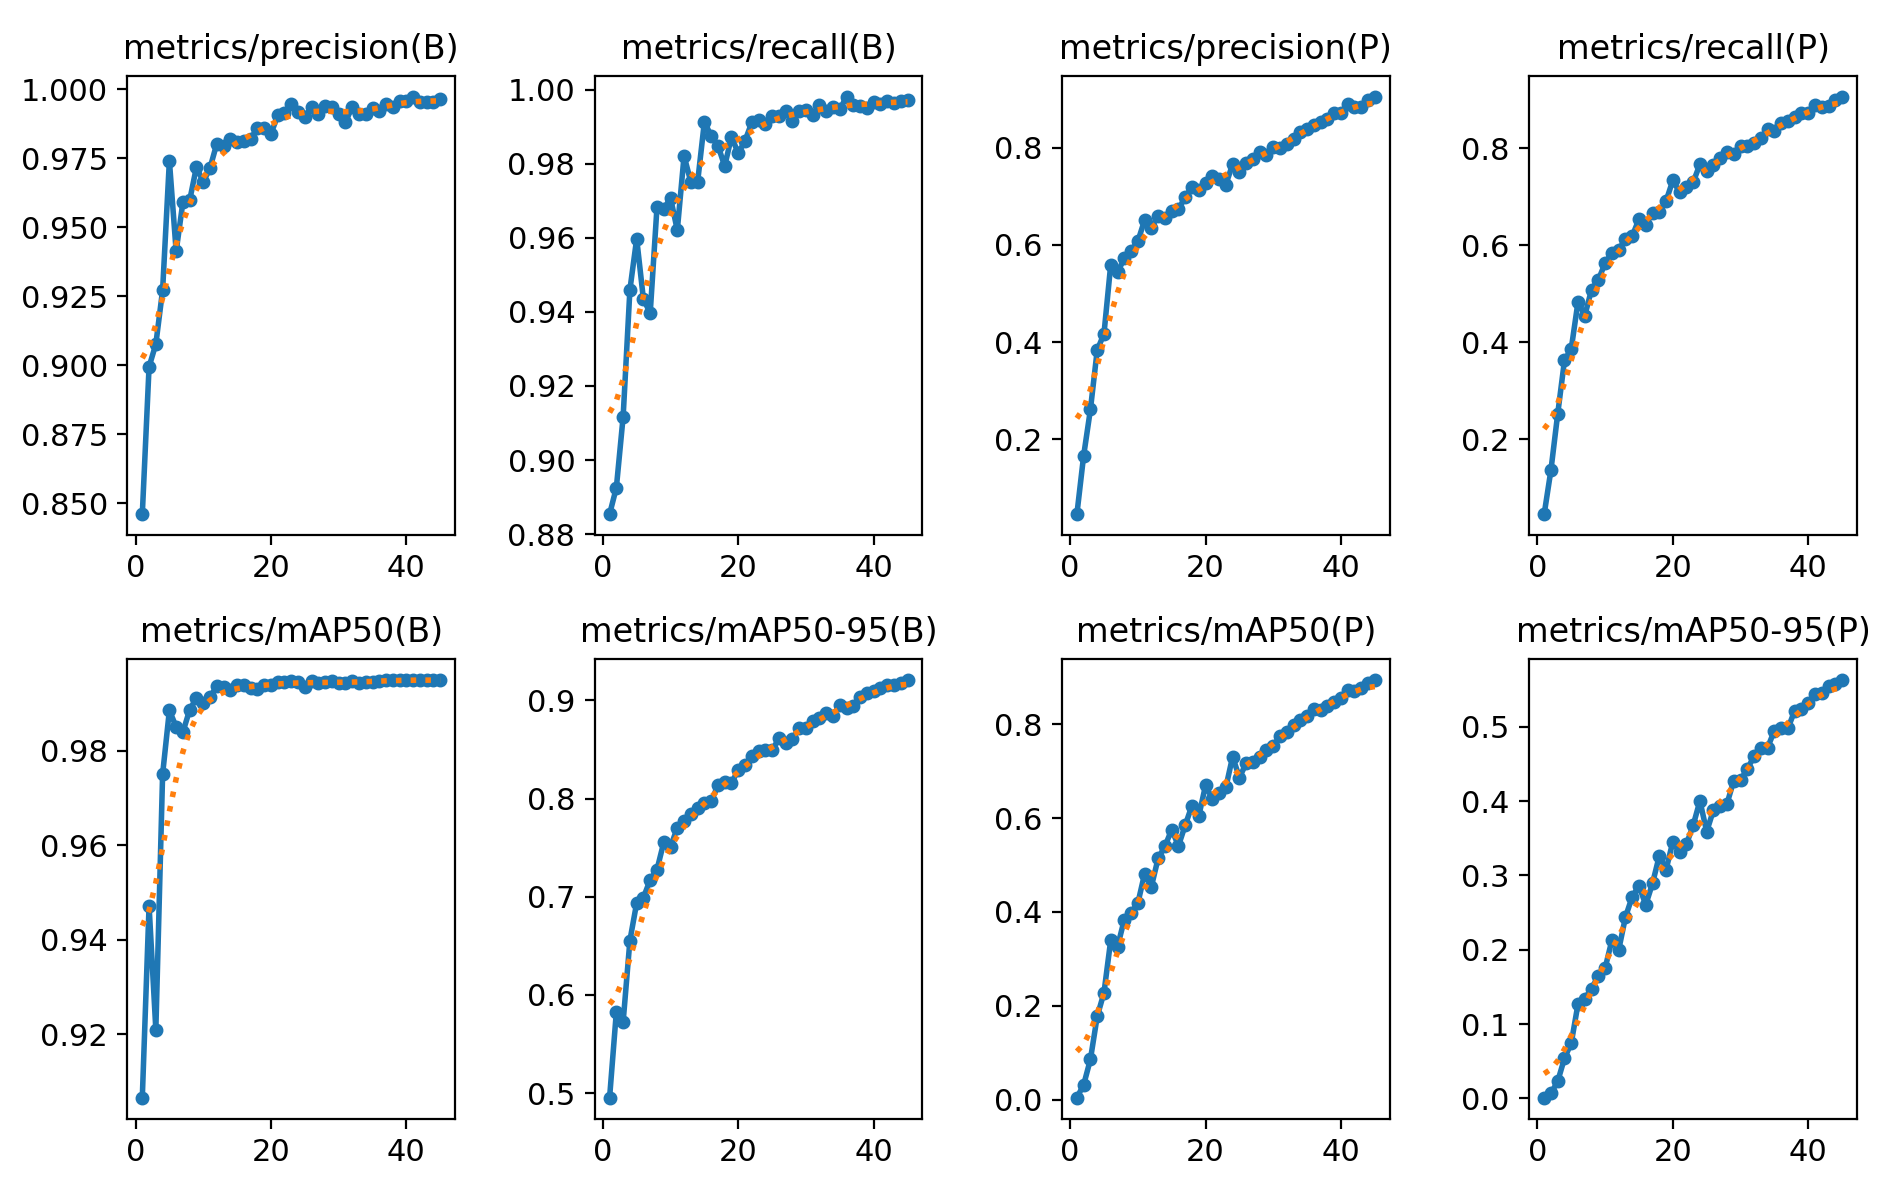
\includegraphics[width=1.0\textwidth,keepaspectratio]{Figures/results.png}
\caption[Lokalizační metriky YOLO modelu]{Lokalizační metriky YOLO modelu}
\label{fig:yoloresults}
\end{figure}

Z obrázku \ref{fig:yoloresults} je patrné, že metriky pro lokalizaci klíčových bodů se stále inkrementálně zlepšovaly. Bohužel, v rámci této práce se po dosažení přednastavené hodnoty trénovaných epoch nepovedlo navrátit stav optimalizátoru a plánovače rychlosti učení do stavu, kdy by mohl trénink efektivně a spolehlivě pokračovat.

V rámci evaluace lokalizace byl parametr $\sigma$ pro metriku OKS nastaven na $\sigma=0,05$. Volba hodnoty je v rozsahu hodnot $\sigma$ z dat pro odhad lidské pózy COCO \cite{dutta2023oks}. Výsledky na základě testovací množiny jsou následující:

\begin{table}[hb]
    \centering
    \begin{tabular}{@{}l r @{\hspace{2cm}} l r@{}}
        \toprule
        \multicolumn{2}{l}{\textbf{Detekce (Box)}} & \multicolumn{2}{l}{\textbf{Odhad pózy (Pose)}} \\
        \cmidrule(lr){1-2} \cmidrule(lr){3-4}
        Metrika & {Hodnota} & Metrika & {Hodnota} \\
        \midrule
        Přesnost (P) & 0,995 & Přesnost (P) & 0,757 \\
        Úplnost (R) & 0,991 & Úplnost (R) & 0,732 \\
        mAP@0,5 & 0,995 & mAP@0,5 OKS & 0,730 \\
        mAP@0,5:0,95 & 0,909 & mAP@0,5:0,95 OKS & 0,435 \\
        \bottomrule
    \end{tabular}
    \caption{Přesnost detekce a lokalizace modelu YOLOv11-s}
    \label{tab:vysledky_test}
\end{table}

Z tabulky \ref{tab:vysledky_test} je patrné, že detekce a odhad ohraničujících boxů dosahuje vysokých hodnot všech měřených metrik přesnosti, úplnosti a mAP. Avšak výsledky jsou nejzajímavější pro odhad pózy (lokalizaci), kde průměrná přesnost nad prahem 0,5 dosahuje zhruba 0,730. Přísnější metrika mAP@0,5 však dosahuje zhruba přesnosti 0,435. Po vizuální inspekci inferenčních výsledků s nízkou hodnotou mAP se dá usoudit, že na vině jsou primárně snímky s neúplným modelem v záběru. Na lokálním systému jsme dosáhli následujících průměrných inferenčních rychlostí:

\begin{table}[ht]
    \centering
    \begin{tabular}{@{}l l l r}    
    \toprule
    Předzpracování & Inference & Post-zpracování & Velikost vstupu \\
    1,0 ms & 11,8 ms & 1,8 ms & $640\times384\times3$ \\
    \end{tabular}
    \caption{Rychlost inference modelu YOLOv11-s}
    \label{tab:rychlost_yolo}
\end{table}